
\chapter{\enginline{1}. ಮೊದಲ ಮಾತು}

ಹೆಚ್ಚಿನವರು ಯೋಗಾಭ್ಯಾಸವನ್ನು ಆರಂಭಿಸುವುದು ಅದು ಜೀವನದಲ್ಲಿ ಅತ್ಯಗತ್ಯ ವೆಂದು ತೋರಿಬಂದಾಗ. ನಾನು ಸಹ ಅದಕ್ಕೆ ಅಪವಾದವಲ್ಲ. ಎಳೆತನದಲ್ಲಿ ಕೆಲವೆಲ್ಲ ಯೋಗಾಭ್ಯಾಸಗಳನ್ನು ನಾನು ಕಲಿತಿದ್ದೆ. ಆದರೂ ಅವನ್ನು ನಾನು ಕ್ರಮಬದ್ಧವಾಗಿ ನಿತ್ಯ ನಡೆಸುತ್ತಿರಲಿಲ್ಲ. ನನಗದರ ಮಹತ್ವದ ಅರಿವೂ ಅಷ್ಟಿದ್ದಿಲ್ಲ, ಸಮಯವೂ ದೊರಕುತ್ತಿರಲಿಲ್ಲ.

ಆದರೆ ಕ್ರಮೇಣ ನನಗೆ ಸಾಮಾನ್ಯ \enginline{40} ರ ವಯಸ್ಸು ಬಂದಿತು. ಆಗ ಬೌದ್ಧಿಕ ಹಾಗೂ ಮಾನಸಿಕ ಕೆಲಸದ ಒತ್ತಡದಿಂದ ಬರುವ ಆಯಾಸ, ನೋವು ತಲೆದೋರ ಲಾರಂಭಿಸಿತು. ನಾನಾಗ ಮೆಡಿಕಲ್ ಕಾಲೇಜಿನ ಹಾಗೂ ದೊಡ್ಡ ಆಸ್ಪತ್ರೆಯ ನಿರ್ದೇಶಕನಾಗಿದ್ದೆ. ಮಾತ್ರವಲ್ಲದೆ ವಿಶ್ವವಿದ್ಯಾನಿಲಯದ ತಾತ್ಕಾಲಿಕ ಉಪಕುಲಪತಿ ಸಹ ಆಗಿದ್ದೆ. ಆಗಾಗ್ಗೆ—ಬಿರುಸಾದ ಎದೆಬಡಿತ ತೋರುವುದು, ಕೆಲಸ ಮಾಡುವಾಗ ಮೇಲುಸಿರು ಬರುವುದು, ಸರಿಯಾಗಿ ನಿದ್ರೆ ಬಾರದಿರುವುದು ಮುಂತಾದವುಗಳೆಲ್ಲ ಒಂದೊಂದಾಗಿ ತಲೆದೋರಲಾರಂಭಿಸಿದುವು. ಆಗ ನನಗೆ ಈ ಯೋಗಾಭ್ಯಾಸ ವಿಷಯದಲ್ಲಿ ಆಸಕ್ತಿ ಮೂಡಿಬರತೊಡಗಿತು. ಆ ಸಂದರ್ಭದಲ್ಲಿ ಸಹ, ಮೇಲೆ ಹೇಳಿದ ಒತ್ತಡದ ನೋವು ಕಾವುಗಳು ಕಾಡತೊಡಗಿದೊಡನೆಯೇ ನಾನೀ ಯೋಗ ಭ್ಯಾಸವನ್ನು ಆರಂಭಿಸಲಿಲ್ಲ. ಈ ನೋವು ಆರಂಭವಾದಾಗ ನಮ್ಮ ವೈದ್ಯತಜ್ಞರು ಎಲ್ಲರಂತೆಯೇ ನನಗೂ ಬೇರೆಬೇರೆ ತರದ ಹೊಸ ಶಾಮಕಮಾತ್ರೆಗಳನ್ನು \enginline{(Tranquilisers)} ಕೊಡಲಾರಂಭಿಸಿದರು. ಆದರೆ, ಅದರ ಪರಿಣಾಮವಾಗಿ ಮನಸ್ಸಿಗೆ ಒಂದು ತರದ ಮಂಕು, ದಿನವಿಡೀ ಜೊಂಪು ತಲೆದೋರತೊಡಗಿತು. ಅಷ್ಟೇ ಅಲ್ಲದೆ ಆ ಮಾತ್ರೆಗಳನ್ನು ನಿಲ್ಲಿಸದೊಡನೆ ಆ ಹಳೆಯ ನೋವುಗಳೆಲ್ಲ ಮತ್ತಷ್ಟು ಜೋರಾಗಿ ಕಾಡತೊಡಗಿದುವು. ಹಾಗಾಗಿ ಈ ಔಷಧಿಗಳ ವಿಚಾರದಲ್ಲಿ ನನಗೆ ಜುಗುಪ್ಸೆ ಸಹ ಉಂಟಾಯಿತು. ಹಾಗಾದರೆ ಮತ್ತೇನು ಮಾಡುವುದು?

ಹೀಗೆ ನಾನು ಜೀವನದಲ್ಲೇ ಬೆಂದು ಬೇಸತ್ತುಹೋಗಿದ್ದೆ. ಆಗ ನನ್ನ ಆಪ್ತ ಸಹೋದ್ಯೋಗಿಯೊಬ್ಬರು—ನೀವೇಕೆ ಯೋಗಾಭ್ಯಾಸವನ್ನಾರಂಭಿಸಬಾರದು? ಆ ಮೂಲಕ ದೈಹಿಕಮಾನಸಿಕ ಶಕ್ತಿಯನ್ನು ಪುನರ್ನವೀಕರಿಸಿಕೊಂಡು, ದುಡಿದು ಜೀವನದ ಸಾರ್ಥಕತೆಯನ್ನು ಸಾಧಿಸಬಾರದು—ಎಂದು ಮೊದಲಾಗಿ ಮೆಲ್ಲನೆ ಸೂಚಿಸಿದರು.

ಈ ಹಿತನುಡಿಯಂತೆ, ನಾನು ಮನಸ್ಸಿಲ್ಲದ ಮನಸ್ಸಿನಿಂದ ಕೆಲ ಯೋಗಾ ಭ್ಯಾಸಗಳನ್ನಾರಂಭಿಸಿದೆ. ಎಳೆತನದಲ್ಲೇ ಈ ಯೋಗದ ಕೆಲವು ರೀತಿನೀತಿಗಳನ್ನು ನಾನು ಕಲಿತಿದ್ದೆ. ಹಾಗಾಗಿ ಬೆಳಗ್ಗೆದ್ದು ಪ್ರತಿದಿನ ನಾಲ್ಕು ಮೂಲಭೂತ ಯೋಗಾ ಭ್ಯಾಸಗಳನ್ನು ನಡೆಸತೊಡಗಿದೆ. ಒಬ್ಬ ತಜ್ಞ ಗುರುವನ್ನು ಕಂಡು ನಾನು ಮಾಡುತ್ತಿ ರುವ ಯೋಗಾಭ್ಯಾಸ ಸರಿಯಾದ ರೀತಿಯಲ್ಲಿದೆ ಎಂದೂ ಖಚಿತಪಡಿಸಿಕೊಂಡೆ.

ಒಂದೇ ವಾರದೊಳಗೆ ನನ್ನ ದೈಹಿಕಮಾನಸಿಕ ಪರಿಸ್ಥಿತಿಯಲ್ಲಿ ಸುಧಾರಣೆ ತೋರಲಾರಂಭಿಸಿತು. ನನಗೆ ಈ ವಿಚಾರದಲ್ಲಿ ವಿಸ್ಮಯವಾಗುವಂತಾಯಿತು. ನನ್ನ ದೇಹದೊಳಗೆ ಅಪಾರಶಕ್ತಿ ತುಂಬಿದೆ! ನನ್ನ ಆರೋಗ್ಯವನ್ನು ಉತ್ತಮಪಡಿಸಿಕೊಂಡು ಆ ಶಕ್ತಿಯನ್ನು ನಾನು ಧಾರಾಳ ಬಳಸಿಕೊಳ್ಳಬಹುದು ಎಂದು ನನಗೇ ತೋರ ಲಾರಂಭಿಸಿತು.

ಕ್ರಮೇಣ, ನಾನೇ ಈ ಯೋಗಾಭ್ಯಾಸವನ್ನು ಪ್ರತಿದಿನವೂ ನಿಯತರೀತಿಯಲ್ಲಿ ನಿಷ್ಠೆಯಿಂದ ಮುಂದುವರಿಸಿದೆ. ಪರಿಣಾಮವಾಗಿ ನನ್ನ ನೋವುಕಾವುಗಳಾದ ಎದೆ ಡವಡವಗುಟ್ಟುವುದು, ನಿದ್ರೆ ಬಾರದಿರುವುದು, ನಿಷ್ಕಾರಣ ಕಳವಳ—ಮಂತಾದು ವೆಲ್ಲ ಕ್ರಮೇಣ ಕಡಿಮೆಯಾದವು. ಅದರೊಂದಿಗೆಯೇ ನನ್ನ ದೇಹಸ್ಥಿತಿ, ಕಾರ್ಯ ದಕ್ಷತೆಗಳೂ ಸುಧಾರಿಸಲಾರಂಭಿಸಿದುವು. ವೃದ್ಧಾಪ್ಯದ ಲಕ್ಷಣಗಳಾದ ಆಯಾಸ, ತಲೆಗೂದಲ ಉದುರುವಿಕೆ, ಮೊದಲಾದವುಗಳೆಲ್ಲ ತಡೆಗಟ್ಟಲ್ಪಟ್ಟಂತಾದುವು. ಹಾಗೆಯೇ ಮೈಚರ್ಮದ ಸುಕ್ಕುಗಟ್ಟುವಿಕೆ, ಅದರಲ್ಲೂ ಮುಖ್ಯವಾಗಿ ಮುಖದ ಮೇಲಿನ ನೆರಿಗೆ, ಹಲ್ಲುಗಳ ಸಡಿಲಾಗುವಿಕೆ, ಮೊದಲಾದವು ಸಹ ಕಡಿಮೆಯಾಗ ತೊಡಗಿದುವು. ಇವೆಲ್ಲಕ್ಕಿಂತಲೂ ಮುಖ್ಯವಾಗಿ ನನ್ನಲ್ಲಿ ಒಂದು ತರದ ಹೊಸ ಚೈತನ್ಯದ ಉದಯವಾದಂತಾಯಿತು. ಅದರಿಂದಾಗಿ ನನ್ನ ಈ ಹೊಸ ಶಕ್ತಿಯನ್ನು ಹೊಸಹೊಸ ಬೌದ್ಧಿಕ, ರಚನಾತ್ಮಕ ಚಟುವಟಿಕೆಗಳಲ್ಲಿ ವಿನಿಯೋಗಿಸಲು ಅನು ಕೂಲವಾಗುವಂತೆಯೂ ಆಯಿತು. ಈ ನನ್ನ ಗುಪ್ತಸಾಮರ್ಥ್ಯವನ್ನು ಧಾರಾಳ ಉಪಯೋಗಿಸಲು ಸಾಧ್ಯವಾದ್ದರಿಂದ ನನ್ನ ಸಾಧನೆಗಳೆಲ್ಲ ಮೊದಲಿಗಿಂತಲೂ ಉತ್ತಮ ಮಟ್ಟಕ್ಕೆ ಏರುವಂತಾಯಿತು. ನನ್ನ ಸಮಾನವಯಸ್ಕರಿಗಿಂತ ಹೆಚ್ಚಿನ ಮಟ್ಟದಲ್ಲಿ ನಾನು ದುಡಿಯುವಂತೆಯೂ ಆಯಿತು.

ಈ ಸಂದರ್ಭದಲ್ಲಿ 'ಗುಪ್ತಸಾಮರ್ಥ್ಯ'—ಎಂಬೀ ಪ್ರಮುಖ ಅಂಶವನ್ನು ಒತ್ತಿಹೇಳಬೇಕಾಗಿದೆ. ಏಕೆಂದರೆ ಹೆಚ್ಚಿನವರು ತಮ್ಮ \enginline{40} ಅಥವಾ \enginline{50} ನೇ ವಯಸ್ಸಾಗುವ ವೇಳೆಗೇ ಸೋತು ಸುಣ್ಣವಾಗುತ್ತಾರೆ; ತಮ್ಮ ರಚನಾತ್ಮಕ ಚಟುವಟಿಕೆ ಗಳನ್ನೆಲ್ಲ ತೊರೆದುಬಿಡುವ ನಿರಾಶಾವಾದಿಗಳಾಗುತ್ತಾರೆ. ಆದರೆ, ಯೋಗಾಭ್ಯಾಸದ ಪರಿಪಾಲನೆಯಿಂದಾಗಿ ಹೊಸ ಚೈತನ್ಯ ಪಡೆಯಲು ಸಾಧ್ಯವಿದೆ; ವಯಸ್ಸೆಷ್ಟೇ ಆಗಲಿ, ತನ್ನ ಜೀವಮಾವಿಡೀ ಬೌದ್ಧಿಕ ಚಟುವಟಿಕೆಗಳನ್ನೆಲ್ಲ ಮೊದಲಿನಂತೆಯೇ ಮುಂದುವರಿಸಿಕೊಂಡು ಹೋಗಲು ಸಾಧ್ಯವಿದೆ—ಎಂಬೀ ಅಂಶ ಹೆಚ್ಚಿನವರಿಗೆ ತಿಳಿದಿಲ್ಲ. ಆದರೆ, ಸ್ವಾನುಭವದಿಂದ ಹೇಳುವುದಿದ್ದರೆ, ಈ ಯೋಗಸಾಮರ್ಥ್ಯ ವಿಚಾರದಲ್ಲಿ ಸಂದೇಹಪಡಲು ಕಾರಣವೇ ಇಲ್ಲ.

ಹೀಗೆ, ಯೋಗಾಭ್ಯಾಸದಿಂದ ಒದಗುವ ಅಪಾರ ಸಾಮರ್ಥ್ಯದ ಕಾರಣ ದಿಂದಾಗಿಯೇ ಇಂದು ಜಗತ್ತಿನ ಎಲ್ಲ ಮೇಧಾವಿಗಳೂ ಈ ಯೋಗದತ್ತ ಆಕರ್ಷಿತ ರಾಗಿದ್ದಾರೆ. ಇದು ಅತ್ಯಂತ ಜನಪ್ರಿಯವೂ ಆಗಿದೆ. ಪ್ರಪಂಚದ ಎಲ್ಲ ಮೂಲೆ ಮೂಲೆಗಳಲ್ಲೂ ಯೋಗಭ್ಯಾಸ ತರಬೇತಿ ಕೇಂದ್ರಗಳು ತಲೆ ಎತ್ತಿ ಇದರ ಪ್ರಸಾರ ಕಾರ್ಯ ಸಾಗುತ್ತಿದೆ. ಅದಕ್ಕಾಗಿ ಟಿ.ವಿ., ರೇಡಿಯೋ, ಪತ್ರಿಕೆ, ಪುಸ್ತಕ—ಮುಂತಾದು ವನ್ನು ಬಳಸುತ್ತಾರೆ. ಇದರ ಪ್ರಯೋಜನವನ್ನು ಪ್ರಸಾರಗೈಯುತ್ತಾರೆ.

ಭಾರತದಲ್ಲಿ ಸಹ ಎಷ್ಟೋ ಶಿಕ್ಷಣ ಸಂಸ್ಥೆಗಳಲ್ಲಿ ಈ ಯೋಗಾಭ್ಯಾಸವನ್ನು ಕಡ್ಡಾಯಗೊಳಿಸಿದ್ದಾರೆ. ಇನ್ನೆಷ್ಟೋ ವಿದ್ಯಾಲಯಗಳಲ್ಲಿ ಐಚಿ, ಕವಾಗಿ ಇದನ್ನು ಅಭ್ಯಾಸ ಮಾಡಲಿಕ್ಕೆ ತಕ್ಕ ವ್ಯವಸ್ಥೆ ಗೈದಿದ್ದಾರೆ. ಇತ್ತೀಚೆಗೆ ಅಮೆರಿಕದಲ್ಲಿ ಒಂದು ಹೊಸ ವಿಶ್ವವಿದ್ಯಾಲಯವನ್ನೇ ಇದಕ್ಕಾಗಿ ಕೆಲ ಉತ್ಸಾಹೀ ಕಾರ್ಯಕರ್ತರು ಆರಂಭಿ ಸಿದ್ದಾರೆ. ಅಲ್ಲಿ ಯೋಗಾಭ್ಯಾಸದ ವಿಧಾನ ಹಾಗೂ ಪ್ರಯೋಜನಗಳ ಸಮಗ್ರ ಪರಿಶೀಲನೆಗೈಯುವ ವ್ಯವಸ್ಥೆ ಮಾಡಿದ್ದಾರೆ. ಈ ಯೋಗಾಭ್ಯಾಸವನ್ನು ಹಲವಾರು ಮಾನಸಿಕ ಹಾಗೂ ದೈಹಿಕ ಕಾಯಿಲೆಗಳನ್ನು ತಡೆಗಟ್ಟಲು ಒಂದು ಉತ್ತಮ ಸಾಧನವನ್ನಾಗಿ ಸಹ ಪ್ರಪಂಚದಾದ್ಯಂತ ಇತ್ತೀಚೆಗೆ ಬಳಸುತ್ತಿದ್ದಾರೆ. ಸಾಮಾನ್ಯ ಮನೋವೈಕಲ್ಯದಂತಹ \enginline{(Mental aberration)} ರೋಗಗಳನ್ನು ಹಿಡತಕ್ಕೆ ತರಲಂತೂ ವಿಶೇಷತಃ ಇದನ್ನು ಉಪಯೋಗಿಸುತ್ತಾರೆ.

ಹೀಗೆ ಆಧುನಿಕ ಮಾನವನ ನರಳಾಟವನ್ನು ಕಡಿಮೆ ಮಾಡಲಿರುವ ಯೋಗಾಭ್ಯಾಸಕ್ಕೆ ಉತ್ತಮ ಭವಿಷ್ಯವಿದೆಯೆಂದು ಧಾರಾಳ ಹೇಳಬಹುದು. ಅದಕ್ಕಾಗಿ ನಾವೆಲ್ಲ ಈ ಯೋಗಕ್ಕೆ ಅವಶ್ಯ ಕೃತಜ್ಞರಾಗಿರಬೇಡವೇ?

ತಜ್ಞರು ಹೇಳುವಂತೆ, ಇತ್ತೀಚಿನ ವರ್ಷಗಳಲ್ಲಿ ಮಾನಸಿಕ ಒತ್ತಡದ ಕಾವು ನೋವುಗಳು ಪ್ರಪಂಚದಾದ್ಯಂತ ಭಯಂಕರ ರೂಪದಲ್ಲಿ ಏರುತ್ತಿವೆ. ಇದನ್ನು ಹಿಡಿತಕ್ಕೆ ತರುವಲ್ಲಿ ಯೋಗಾಭ್ಯಾಸ ಅತ್ಯಂತ ಪರಿಣಾಮಕಾರೀ ಸಾಧನವಾದ್ದರಿಂದ ಇದರ ಅವಶ್ಯಕತೆ ಎಲ್ಲರಿಗೂ ಈಗ ಅರ್ಥವಾಗುತ್ತಿದೆ.

ಇಂದು, ಹೆಚ್ಚಿನ ಸಾಂಕ್ರಾಮಿಕ ರೋಗಗಳನ್ನು ತಡೆಗಟ್ಟಿ ಮರಣ ಸಂಖ್ಯೆಯನ್ನು ನಮ್ಮ ವೈದ್ಯವಿಜ್ಞಾನಿಗಳು ಕುಗ್ಗಿಸಿದ್ದಾರೆ. ಅದರಿಂದಾಗಿ, ಏರುತ್ತಿರುವ ಜನ\enginline{}ಸಂಖ್ಯೆಯೂ ಈ ಒತ್ತಡದ ಕಾವುನೋವುಗಳು ಹೆಚ್ಚುತ್ತಿರುವುದಕ್ಕೆ ಕಾರಣವಿರ ಬಹುದು. ಅಷ್ಟೇ ಅಲ್ಲದೆ ಹೊಸಹೊಸ ದೊಡ್ಡ ಮಟ್ಟದ ಕೈಗಾರಿಕೆಗಳ ಆರಂಭ

\begin{center}
ಪಶ್ಚಿಮ ಜರ್ಮನಿ
\end{center}


\begin{figure}
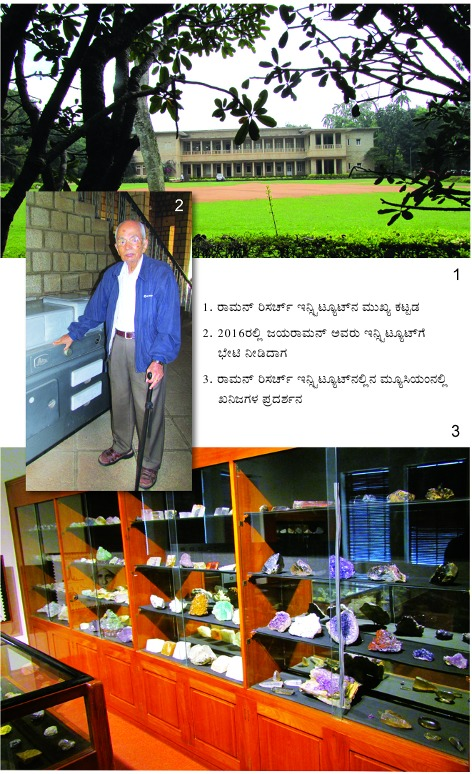
\includegraphics{images/001.jpg}
\caption{ಚಿತ್ರ \enginline{1: 1952} ರಿಂದ \enginline{58} ರ ವರೆಗಿನ ಆರು ವರ್ಷಗಳಲ್ಲಿ ವರ್ಷದಿಂದ ವರ್ಷಕ್ಕೆ ಏರುತ್ತಹೋದ ಮರಣಸಂಖ್ಯೆ ಕಾಣಬಹುದು.}
\end{figure}

ಪಶ್ಚಿಮ ಜರ್ಮನಿಯಲ್ಲಿ ಹೃದಯಾಘಾತದಿಂದ ಸಾಯುವವರು, \enginline{1952} ರಲ್ಲಿ \enginline{15} ಸಾವಿರವಾದರೆ \enginline{58} ರಲ್ಲಿ \enginline{30} ಸಾವಿರಕ್ಕೇರಿ ಇಮ್ಮಡಿಯಾಗಿದ್ದಾರೆ.

ದಿಂದಾಗಿ ಮಹಾಮಹಾ ನಗರಗಳು ತಲೆ ಎತ್ತುತ್ತಿವೆ. ಜನನಿಬಿಡವಾದ ಕುಲುಷಿತ ವಾತಾವರಣ ಇಂದು ಎಲ್ಲೆಡೆ ಬೆಳೆದು ಬರುತ್ತಿದೆ. ಮಾನವ ಪ್ರಶಾಂತ ಜೀವನ ನಡೆಸಲು ಅಸಾಧ್ಯವಾದ ಪರಿಸ್ಥಿತಿ ಬಂದೊದಗಿದೆ. ಇದೂ ಮಾನಸಿಕ ತುಮುಲಗಳ ಹೆಚ್ಚಳಕ್ಕೆ ಕಾರಣವಿರಬಹುದು. ಅಂತು ಈ ಯುಗದ ದೊಡ್ಡ ಮಾರಕರೋಗ, ಮಾನಸಿಕ ಒತ್ತಡದ ಕಾವುನೋವು ಎಂಬುದನ್ನು ಎಲ್ಲರೂ ಒಪ್ಪಿರುತ್ತಾರೆ.

ಮಿತಿಮೀರಿದ ಒತ್ತಡದ ಕಾಯಿಲೆಗಳಿಗೆ ಕಾರಣವಾದ ಅಂಶಗಳನ್ನು ದೂರಗೈಯುವ ಕಾರ್ಯಕ್ರಮಗಳನ್ನು ಇಂದು ಸಮಾಜ ಹಾಗೂ ಸರ್ಕಾರ ಕೈಗೊಳ್ಳ ಬೇಕಾಗಿದೆ. ಅದರೊಂದಿಗೆಯೇ ಜನಸಾಮಾನ್ಯರು ಯೋಗಾಭ್ಯಾಸವನ್ನೂ ಆರಂಭಿಸಿ ದ್ದಾದರೆ ಅಂತಹ ಕಾವುನೋವುಗಳು ವಿಶೇಷವಾಗಿ ತಲೆದೋರದಂತಾಗಬಹುದು; ಮಾತ್ರವಲ್ಲದೆ ಬಂದೊದಗಿದ ನೋವನ್ನು ತಡೆಗಟ್ಟಲೂ ಸಾಧ್ಯವಾಗಬಹುದು. ಹೀಗೆ ಯೋಗವು ಸಮಾಜಹಿತಕ್ಕಿರುವ ಪ್ರಭಾವಶಾಲೀ ಸಾಧನ ಎಂಬುದನ್ನು ನಾವು ಧೈರ್ಯದಿಂದ ಹೇಳಬಹುದಾಗಿದೆ.

ಯೋಗದಿಂದೊದಗುವ ಪ್ರಯೋಜನ ಧಾರಾಳವಾಗಿದೆ ಎಂದು ತಿಳಿದು ಬಂದಿದೆ ನಿಜ. ಆದರೆ ಯೋಗಾಭ್ಯಾಸವು ದೇಹದೊಳಗೆ ಯಾವ ರೀತಿಯಲ್ಲಿ ತನ್ನ ಪ್ರಭಾವ ಬೀರುತ್ತದೆ ಎಂಬುದರ ವೈಜ್ಞಾನಿಕ ಪರಿಶೀಲನೆ ನಡೆಸುವಲ್ಲಿ ಹೆಚ್ಚಿನ ಸಂಶೋಧನೆ ನಡೆದಂತಿಲ್ಲ. ಯೋಗದ ಪರಿಣಾಮ ವಿಚಾರವಾಗಿ ಅಪಹಾಸ್ಯ ಗೈಯು ವವರೂ ಕೆಲವರಿದ್ದಾರೆ. ತಕ್ಕರೀತಿಯಲ್ಲಿ ಮಾಡದ ಹಠಯೋಗದಿಂದ ಒದಗುವ ಅನಿಷ್ಟ ಪರಿಣಾಮಗಳನ್ನು ದೊಡ್ಡದು ಮಾಡುವವರೂ ಇನ್ನೂ ಕೆಲವರಿದ್ದಾರೆ. ಅಷ್ಟೇಅಲ್ಲದೆ, ಯೋಗಾಭ್ಯಾಸದ ಸತ್ಪರಿಣಾಮ ಯಾವುದೋ ಒಂದು ಅವ್ಯಕ್ತ ಶಕ್ತಿಯಿಂದಾಗಿ ಒದಗುತ್ತದೆ; ಆ ಕಾರಣ ಈಗಿನ ವೈಜ್ಞಾನಿಕ ಸಾಧನಗಳಿಂದ ಅವನೆಲ್ಲ ಅಳೆದು ಹೇಳಬರುವುದಿಲ್ಲ ಎಂದು ಹೇಳುವವರೂ ಇದ್ದಾರೆ. ಮತ್ತೆ ಕೆಲವರು, ಯೋಗಾಭ್ಯಾಸದಿಂದ ಆಧ್ಯಾತ್ಮಿಕಶಕ್ತಿ ಹೆಚ್ಚುವ ಕಾರಣ ದೇಹಮನಸ್ಸು ಗಳು ಸುದೃಢಗೊಳ್ಳುತ್ತವೆ; ಈಗಿನ ವೈಜ್ಞಾನಿಕ ಉಪಕರಣಗಳಿಂದ ಅವನ್ನೆಲ್ಲ ಪರಿಶೀಲಿಸಲಾಗುವುದಿಲ್ಲ ಎಂದೂ ಹೇಳುತ್ತಾರೆ. ಇಂತಹ ಅಭಿಪ್ರಾಯ ಹಲವೆಡೆ ಇರುವುದಾದರೂ ಯೋಗಾಭ್ಯಾಸದಿಂದ ಉತ್ತಮ ಪ್ರಯೋಜನವಿದೆ ಎಂಬ ವಿಚಾರ ದಲ್ಲಿ ಹೆಚ್ಚಿನ ಭಿನ್ನಾಭಿಪ್ರಾಯವಿಲ್ಲ. ಆದರೆ ಅದು ಹೇಗೆ ದೇಹಮನಸ್ಸುಗಳಲ್ಲಿ ತನ್ನ ಪ್ರಭಾವ ಬೀರುತ್ತದೆ ಎಂಬಂಶ ಮಾತ್ರ ಇನ್ನೂ ಒಂದು ತರದ ರಹಸ್ಯವಾಗಿಯೇ ಹೆಚ್ಚಿನವರಲ್ಲಿ ಉಳಿದಿದೆ.

ಈ ಒಂದು ಹಿನ್ನೆಲೆಯಲ್ಲಿ, ಸಮಸ್ಯೆಯನ್ನು ನಿಷ್ಪಕ್ಷಪಾತವಾದ ವೈಜ್ಞಾನಿಕ ರೀತಿಯಲ್ಲಿ ಪರಿಶೀಲಿಸಬೇಕು; ಯೋಗಾಭ್ಯಾಸ ಪ್ರತಿಯೊಂದು ಹಂತದಲ್ಲೂ ಹೇಗೆ ಕಾರ್ಯಕಾರಿಯಾಗುತ್ತದೆ; ಎಂಬುದನ್ನು ವಿವರವಾಗಿ ಮತ್ತು ವೈಜ್ಞಾನಿಕವಾಗಿ ಕಂಡುಹಿಡಿಯಬೇಕು ಎಂದು ನಾವು ನಿರ್ಧರಿಸಿದೆವು. ದೇಹಮನಸ್ಸುಗಳ ಅವ್ಯಕ್ತ ಸಂಕರದೊಳಗೆ ನಡೆಯುವ ಯೋಗಾಭ್ಯಾಸದ ಪರಿಣಾಮವನ್ನು ವೈಜ್ಞಾನಿಕವಾಗಿ ಅಳೆದು ನೋಡಲು ಸಾಧ್ಯವಾಗಬಹುದೇ ಎಂಬ ಸಂದೇಹವೂ ಮೊದಲು ನಮ್ಮನ್ನು ಆವರಿಸಿತ್ತು. ನಾನಾ ರೀತಿಯಲ್ಲಿ ಪ್ರಯತ್ನಿಸಿದ ಮೇಲೆ, ಯೋಗವನ್ನು ಸರಿಯಾದ ರೀತಿಯಲ್ಲಿ ನಿಶ್ಚಿತ ಅವಧಿಯವರೆಗೆ ಅಭ್ಯಾಸ ಮಾಡಿದ ಪ್ರತಿಯೊಬ್ಬ ವ್ಯಕ್ತಿಯನ್ನೂ ವೈಜ್ಞಾನಿಕ ಪರೀಕ್ಷೆಗೊಳಪಡಿಸಿದೆವು. ಆಗ ಮೂಡಿಬಂದ ಅದರ ಸತ್ಪರಿಣಾಮವನ್ನು ವೈಜ್ಞಾನಿಕ ರೀತಿಯಲ್ಲಿ ಪರಿಶೀಲಿಸಿ ಅಳೆದು ನೋಡಲು ಸಾಧ್ಯವಾಯಿತು. ಆಗ ವಿಸ್ಮಯ ಹಾಗೂ ಸಂತೋಷವೂ ಉಂಟಾಯಿತು. ಈ ವಿಚಾರವನ್ನು ಯಾವ ವಿಧದಲ್ಲಿ, ವೈಜ್ಞಾನಿಕವಾಗಿ ಅಳೆದು ನೋಡಿದೆವು; ಹಾಗೂ ಅದು ಹೇಗೆ ಒಳ್ಳೆಯ ಪರಿಣಾಮವನ್ನುಂಟುಮಾಡುತ್ತದೆ ಎಂದು ಮೊದಲಾದ ಅಂಶವನ್ನು ಮುಂದಿನ ಅಧ್ಯಾಯಗಳಲ್ಲಿ ನಾವು ವಿವರಿಸಲಿದ್ದೇವೆ.

ಯೋಗಾಭ್ಯಾಸವನ್ನು ಮನಃಪೂರ್ವಕವಾಗಿ ಹಾಗೂ ಕ್ರಮಬದ್ಧವಾಗಿ ಪ್ರತಿ ನಿತ್ಯ ಮಾಡಿಕೊಂಡು ಬಂದವರಲ್ಲಿ, ಅತ್ಯಂತ ಉತ್ತಮಮಟ್ಟದ ಫಲಿತಾಂಶ ಉಂಟಾಗಿದೆ ಎಂಬುದು ಮಾತ್ರ ತುಂಬಾ ಸಂತೋಷದ ಸತ್ಯವಿಚಾರ. ಇಷ್ಟು ಮಾತ್ರ ಹೇಳಿದರೆ, ಪ್ರಕೃತಕ್ಕೆ ಸಾಕೆಂದು ತೋರುತ್ತದೆ.

ಈ ಸಂದರ್ಭದಲ್ಲಿ ದೇಹದಣಿಕೆಯ ಈ ಹಠಯೋಗಾಭ್ಯಾಸಕ್ಕೂ, ಆಟೋಟ ಗಾರರು ಮೈದಾನದಲ್ಲಿ ಅಥವಾ ವ್ಯಾಯಾಮಶಾಲೆಯಲ್ಲಿ ನಡೆಸುವ ದೈಹಿಕ ವ್ಯಾಯಾಮಕ್ಕೂ ಏನು ವ್ಯತ್ಯಾಸ ಇದೆ? ಎಂಬೀ ಪ್ರಶ್ನೆ ತಲೆದೋರಬಹುದು. ಪ್ರಾಯಶಃ ಈ ಎರಡರಲ್ಲಿಯೂ ಒಂದಲ್ಲ ಒಂದು ರೀತಿಯ ಮಾಂಸಖಂಡಗಳ ಪ್ರಕ್ರಿಯೆಗಳಿರುವುದರಿಂದ ದೈಹಿಕ ವ್ಯತ್ಯಾಸವಿರಲಾರದು; ಅದರಿಂದ ದೊರಕುವ ಪ್ರಯೋಜನಗಳೂ ಹೆಚ್ಚು ಕಡಿಮೆ ಒಂದೇ ರೀತಿ ಇರಬೇಕು—ಹೀಗೆ ಹೇಳುವುದು ಸಹಜವಾಗಿದೆ.

ದೈಹಿಕ ವ್ಯಾಯಾಮದಿಂದುಂಟಾಗುವ ದೈಹಿಕ ಹಾಗೂ ಜೀವರಾಸಾಯನಿಕ ಬದಲಾವಣೆಗಳ ವಿಚಾರದಲ್ಲಿ ಧಾರಾಳವಾದ ಸಂಶೋಧನೆ ಈ ಮೊದಲೇ ನಡೆದಿದೆ. ಹಾಗಾದ ಕಾರಣ ಈ ಹಠಯೋಗದಿಂದೊದಗುವ ದೇಹಸ್ಥಿತಿಯ ಸುಧಾರಣೆ ವಿಚಾರ ದಲ್ಲಿ ಮತ್ತೊಮ್ಮೆ ಸಂಶೋಧನೆ ನಡೆಸಿ ಪುನರಾವರ್ತನೆ ಮಾಡುವ ಅವಶ್ಯಕತೆ ಇಲ್ಲವೆಂದು ತೋರುತ್ತದೆ.

ಯೋಗಾಭ್ಯಾಸದ ಪ್ರೋತ್ಸಾಹಕರು ಬರೇ ದೈಹಿಕ ವ್ಯಾಯಾಮದಿಂದಾಗುವ ಪರಿಣಾಮಕ್ಕೂ ದೈಹಿಕ–ಮಾನಸಿಕ ಪ್ರಕ್ರಿಯೆಗಳನ್ನೊಳಗೊಂಡ ಸಮಗ್ರ ಯೋಗಾ ಭ್ಯಾಸದ ಪರಿಣಾಮಕ್ಕೂ ತುಂಬಾ ವ್ಯತ್ಯಾಸವಿದೆಯೆಂದು ಹೇಳುತ್ತಾರೆ. ಏಕೆಂದರೆ ದೈಹಿಕ ವ್ಯಾಯಾಮವೆಂದರೆ ಮಾಡಿದ್ದನ್ನೇ ಮಾಡುವ ಸ್ನಾಯುಶಕ್ತಿಯನ್ನು ಬಹಳ ವಾಗಿ ಬಳಸುವ ಪ್ರಕ್ರಿಯೆಯಾಗಿದೆ. ಆದರೆ ಯೋಗಾಭ್ಯಾಸದಲ್ಲಿ ಅಷ್ಟೊಂದು ಸ್ನಾಯುಶಕ್ತಿ ವ್ಯಯವಾಗುವುದಿಲ್ಲ. ಏಕೆಂದರೆ ಯಾವುದಾದರೊಂದು ನಿಶ್ಚಿತ ಸ್ಥಿತಿಯಲ್ಲಿ ಅಂಗಾಂಗಗಳನ್ನು ನಿಲ್ಲಿಸುವ ವಿಧಾನ ಯೋಗಾಭ್ಯಾಸವಾಗಿರುತ್ತದೆ. ಹಾಗೆ ನಿಶ್ಚಿತಸ್ಥಿತಿಯಲ್ಲಿ ದೇಹವನ್ನು ನಿಲ್ಲಿಸಿ, ಸ್ನಾಯುಶಕ್ತಿಯನ್ನು ವಿಶೇಷ ಬಳಸದೆ, ದೇಹ ಮತ್ತು ಮನಸ್ಸಿನ ಶಕ್ತಿಯನ್ನು ಕೇಂದ್ರೀಕರಿಸುವುದು ಯೋಗಾಭ್ಯಾಸದ ತತ್ವವಾಗಿದೆ. ದೈಹಿಕ ವ್ಯಾಯಾಮ ಮಾಡುವಾಗ ಸ್ವಯಂಚಾಲಿತ ಸ್ನಾಯುಗಳಲ್ಲಿ \enginline{(Voluntary Muscles)} ವಿಶೇಷ ರಕ್ತಸಂಚಾರವಾಗುತ್ತದೆ. ಆದರೆ ಯೋಗಾ ಭ್ಯಾಸದಲ್ಲಿ ಸ್ವಯಂಚಾಲಿತ ಸ್ನಾಯುಗಳು, ಅಷ್ಟೊಂದು ದೊಡ್ಡ ಪಾತ್ರವನ್ನು ವಹಿಸು ವುದಿಲ್ಲ. ಬದಲಾಗಿ ಯೋಗಾಭ್ಯಾಸ ದೇಹದ ಮರ್ಮಸ್ಥಾನಗಳ \enginline{(Vital organs)} ರಕ್ತಸಂಚಾರ ಸುಧಾರಣೆಯಲ್ಲಿ ಹೆಚ್ಚಿನ ಪ್ರಭಾವ ಬೀರುತ್ತದೆ. ಉದಾಹರಣೆಗೆ: ಶೀರ್ಷಾಸನ ಮಿದುಳಿನ ನರಮಂಡಲದಲ್ಲಿ ರಕ್ತ ಸಂಚಾರವನ್ನು ಉತ್ತೇಜಿಸುವು ದಾದರೆ, ಸರ್ವಾಂಗಾಸನ ಗಲಗ್ರಂಥಿ ಮತ್ತಿತರ ಅಂತಃಸ್ರಾವೀ ಗ್ರಂಥಿಗಳಲ್ಲಿ \enginline{(Thyroid and other Endocrine Glands)} ರಕ್ತ ಸಂಚಾರವನ್ನು ಉತ್ತಮ ಪಡಿಸುತ್ತದೆ. ಪ್ರಾಣಾಯಾಮ ಹೃದಯ ಮತ್ತು ಶ್ವಾಸಕೋಶಗಳ ರಕ್ತಸಂಚಾರವನ್ನು ಸುಧಾರಿಸುತ್ತದೆ. ಹೀಗೆ ಒಂದೊಂದು ರೀತಿಯ ಯೋಗಾಸನ ಒಂದೊಂದು ಪ್ರಮುಖ ಅಂಗಗಳ ಶಕ್ತಿಯನ್ನು ಉತ್ತಮಪಡಿಸುತ್ತದೆ. ಇದರಿಂದ ಇಡೀ ದೇಹದ ಬೇರಬೇರೆ ಅವಯವಗಳಿಗೆ, ಏಕಕಾಲದಲ್ಲಿ ರಕ್ತ ಸಂಚಾರ ಹೆಚ್ಚಿ ಶಕ್ತಿ ವ್ಯಯ ವಾಗುವ ಸಂಭವ ಇಲ್ಲ. ಹೀಗೆ, ಶಕ್ತಿಯ ಅಪವ್ಯವಗೈಯದೆ, ನಿರ್ದಿಷ್ಟ ಅವಯವದ ನಿಶ್ಚಿತ ಶಕ್ತಿಯನ್ನು ಹೆಚ್ಚಿಸುವುದೇ ಯೋಗಾಭ್ಯಾಸದ ಪ್ರಮುಖ ಉದ್ದೇಶವಾಗಿದೆ.

ಈ ವಿಚಾರದ ವೈಜ್ಞಾನಿಕ ಸಂಶೋಧನೆ ನಡೆಸುವ ಪ್ರಯತ್ನವನ್ನು ನಾವಿಲ್ಲಿ ಕೈಗೊಂಡಿದ್ದೇವೆ. ಅದರ ಫಲಿತಾಂಶವನ್ನು ಅಂಕೆಸಂಖ್ಯೆಗಳ ಮೂಲಕ ಪ್ರಕಟಿಸು ವುದಕ್ಕೆ ಪ್ರಯತ್ನಿಸಿದ್ದೇವೆ. ಆದರೆ ನಮ್ಮ ಪರಿಶೀಲನೆ ಪ್ರಥಮ ಪ್ರಯತ್ನವಾದ ಕಾರಣ, ಇನ್ನೂ ಈ ವಿಚಾರದಲ್ಲಿ ಆಳವಾದ ಸಂಶೋಧನೆ ಮುಂದುವರಿಸಲಿಕ್ಕೆ ಅವಕಾಶವಿದೆ. ಅದಾದಮೇಲೆ ಈ ಯೋಗಾಭ್ಯಾಸವು ಸಾಮಾನ್ಯ ದೈಹಿಕ ವ್ಯಾಯಾಮಕ್ಕಿಂತ ಭಿನ್ನವಾದ ಉತ್ತಮ ಪ್ರಯೋಜನ ಕೊಡಬಲ್ಲುದೆಂಬುದನ್ನು ನಿರ್ದಿಷ್ಟವಾಗಿ ಹೇಳಬಹುದಾಗಿದೆ.

\delimiter

